% fig09_blanket.tex — OpenMC DEMO-class spherical blanket radial build.
% Compiled by the paper Makefile via `make figures` (pdflatex on the snippet).
%
% Data: Appendix E (Tritium breeding), Table "tab:app:geom". 1-D spherical
% radial build [cm], 14.06 MeV DT point source at origin:
%   plasma chamber (vacuum)        0--100   source cavity
%   tungsten (W) armor             100--102 plasma-facing armor (2 cm)
%   EUROFER97 first wall           102--104 RAFM structural FW (2 cm)
%   Pb-15.7Li breeder (90 at% Li6) 104--160 tritium breeding zone (56 cm)
%   SS316 shield                   160--202 neutron/gamma shield (42 cm)
% TBR = 1.3222 +/- 0.0004 (OpenMC 0.15.3 + ENDF/B-VIII.0, 5e6 histories,
% verify atom openmc_tbr_pb157li, PR #1078).
% Drawn as an explicit horizontal radial bar (TikZ rectangles) on a cm axis;
% the inner vacuum cavity (0-100 cm) is shown truncated with a break marker so
% the thin 2 cm W/EUROFER layers stay legible.
%
% Manual single-shot compile (debug):
%   pdflatex -interaction=nonstopmode -halt-on-error fig09_blanket.tex
\documentclass[border=4pt]{standalone}
\usepackage{tikz}
\usetikzlibrary{decorations.pathreplacing}
\begin{document}
% horizontal scale: 1 cm radius -> 0.11 cm on page, offset so r=95 is x origin.
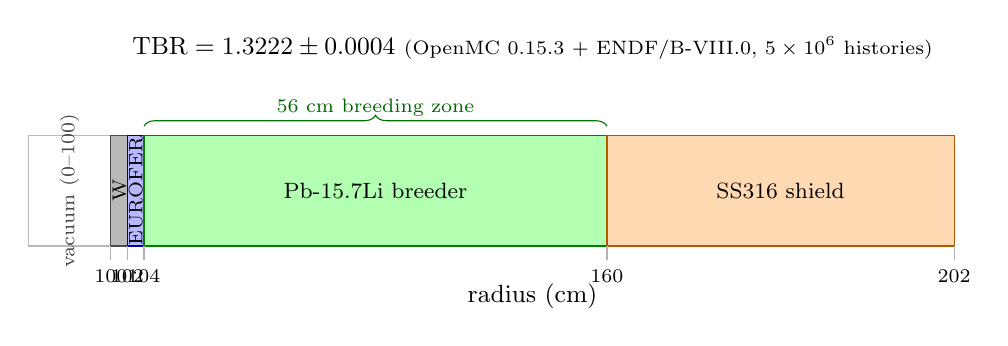
\begin{tikzpicture}[x=0.105cm, font=\footnotesize]
  \def\y{0}      % bar bottom
  \def\h{1.4}    % bar height
  % --- layer rectangles (radius coords, shifted by -95 so r=95 -> 0) ---
  % vacuum cavity (truncated): draw a short stub 90->100 with a break
  \fill[white,draw=gray!55] (-5,\y) rectangle (5,\h);          % 90->100 stub
  \node[gray!55!black,rotate=90,font=\scriptsize] at (0,{\h/2}) {vacuum (0--100)};
  \fill[gray!55,draw=gray!60!black] (5,\y) rectangle (7,\h);   % W 100->102
  \fill[blue!28,draw=blue!55!black] (7,\y) rectangle (9,\h);   % EUROFER 102->104
  \fill[green!30,draw=green!50!black] (9,\y) rectangle (65,\h);% Pb-15.7Li 104->160
  \fill[orange!30,draw=orange!70!black] (65,\y) rectangle (107,\h); % SS316 160->202
  % --- layer labels ---
  \node[rotate=90,font=\scriptsize] at (6,{\h/2}) {W};
  \node[rotate=90,font=\scriptsize] at (8,{\h/2}) {EUROFER};
  \node at (37,{\h/2}) {Pb-15.7Li breeder};
  \node at (86,{\h/2}) {SS316 shield};
  % --- radius axis (ticks at the real interface radii) ---
  \foreach \r/\lab in {5/100,7/102,9/104,65/160,107/202} {
    \draw[gray!60] (\r,\y) -- (\r,{\y-0.18});
    \node[below,font=\scriptsize] at (\r,{\y-0.18}) {\lab};
  }
  \node[below=10pt,font=\small] at (56,\y) {radius (cm)};
  % --- breeder-zone brace (56 cm) ---
  \draw[decorate,decoration={brace,amplitude=4pt},green!45!black]
    (9,{\h+0.12}) -- (65,{\h+0.12})
    node[midway,above,font=\scriptsize,green!40!black] {56 cm breeding zone};
  % --- TBR headline ---
  \node[above,font=\small] at (56,{\h+0.85})
    {$\mathrm{TBR}=1.3222\pm0.0004$ \scriptsize (OpenMC 0.15.3 + ENDF/B-VIII.0, $5\times10^{6}$ histories)};
\end{tikzpicture}
\end{document}
